\chapter*{\textbf{Capítulo II: Marco teórico}}
\label{ch:MarcoTeorico}
\addcontentsline{toc}{chapter}{\textbf{II. Marco teórico}}
\chead{Marco teórico}
\setcounter{chapter}{2}
\setcounter{equation}{0}
\setcounter{figure}{0}
\setcounter{table}{0}

\section*{II.1 Señales observadas por tránsitos de exoplanetas}

\addcontentsline{toc}{section}{II.1 Señales observadas por tránsitos de exoplanetas}

Como se mencionó anteriormente, el método del tránsito es la técnica más popular y exitosa para descubrir nuevos planetas. Un tránsito ocurre cuando un exoplaneta está alineado de manera particular con la línea de observación ($i\sim 90^{\circ}$) y el planeta bloquea parte de la luz de la estrella, lo cual provoca una ligera disminución en su brillo. Como se muestra en la figura 2.1, si $i$ disminuye el tránsito deja de ser visible por el observador, por lo que la probabilidad de observar un tránsito, está en función del ángulo de inclinación con respecto a la perpendicular de la línea de visión.


\begin{figure}[H]
  \centering
    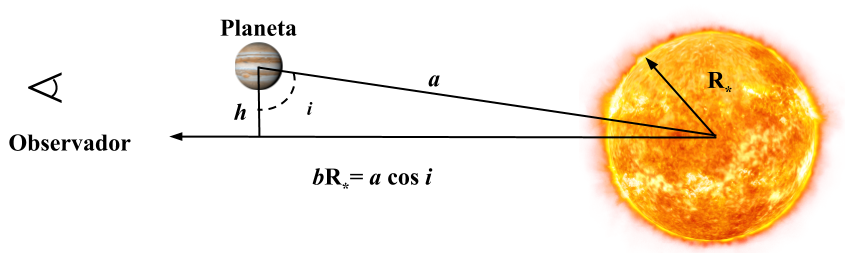
\includegraphics[max size={0.9\textwidth}{0.9\textheight}]{./figures/inclinacion.png}
   \caption{Esquema de un tránsito de exoplaneta observable. $i$ representa la inclinación de la órbita, $R_{*}$ es el radio de la estrella y $b$ el parámetro de impacto.}
    \label{fig_2_1_transito}
\end{figure}


\subsection*{II.1.1 Sistema general de ecuaciones}
\addcontentsline{toc}{subsection}{II.1.1 Sistema general de ecuaciones}

A partir de las señales observadas de tránsitos de exoplanetas, podemos calcular algunas de las propiedades físicas del sistema, teniendo en cuenta las siguientes suposiciones (para este trabajo):

\begin{itemize}
\item La órbita del planeta es circular ($\epsilon = 0$).
\item La masa del planeta es despreciable comparada con la de la estrella anfitriona \\ $M_{p} << M_{*}$.
\item La relación masa-radio de la estrella es conocida.
\item La luz proviene de una sola estrella.
\item No se considerará el oscurecimiento al limbo ($\textit{Limb Darkening}$).
\end{itemize}

Las primeras 3 suposiciones son aceptables para estrellas de secuencia principal, la gran mayoría de los sistemas planetarios cumplen con relaciones similares. Los planetas con periodos orbitales cortos ($\sim 5$ días) tienen excentricidades cercanas a 0.

Bajo estas aproximaciones, podemos describir la curva de luz de un tránsito a partir de 4 ecuaciones. La primera (\ref{ec:profundidadTransito}) representa la profundidad del tránsito $\Delta F$. El flujo total $F$ de una estrella es proporcional a su superficie, el cambio en el flujo debido al tránsito se traduce en el cociente de las áreas de la estrella y el planeta transitando frente a esta.

\begin{equation}
	\label{ec:profundidadTransito}
  \displaystyle \dfrac{\Delta F}{F}=\left(\dfrac{R_*}{R_p} \right)^{2} ;
\end{equation}

De esta relación podemos claramente ver que si conocemos el radio de la estrella $R_{*}$, podemos entonces calcular el radio del planeta $R_{p}$. También esta es la razón por la cual el proyecto \textit{TESS} se enfoca en estrellas pequeñas, porque de esta manera es más sencillo medir $\Delta F$ provocados por planetas más pequeños.

La duración total del tránsito $t_{T}$ está definida por sus parámetros orbitales y el radio estelar.

\begin{equation}
\label{ec:tiempoTransito}
\displaystyle t_{T}=\dfrac{P}{\pi} \mbox{arcsin} \left(\dfrac{R_{*}}{a}\left[ \dfrac{\left( 1+\dfrac{R_{p}}{R_{*}}\right)^{2}-\left( \dfrac{a}{R_{*}} \mbox{cos} i\right)^{2}}{1-\mbox{cos}^{2}i} \right]^{1/2}  \right); 
\end{equation}

esta relación se puede reducir a:

\begin{equation}
\label{ec:tiempoTransitoReduc}
\displaystyle t_{T}=\dfrac{P}{\pi}\sqrt{\left(\dfrac{R_{*}}{a} \right)^{2}- \mbox{cos}^{2}i};
\end{equation}

solo considerando que $a\gg R_{*}\gg R_{p}$ \citep{winn2010transits}, donde $P$ es el periodo orbital dado por la tercera ley de Kepler \ref{ec:kepler3}, $a$ es el semi-eje e $i$ la inclinación de la órbita. Usando $i$, podemos definir $b=\dfrac{a}{R_{*}}\mbox{cos}~i$ conocido como parámetro de impacto, el cual es comúnmente más utilizado para cuantificar la inclinación de la órbita. El periodo orbital se define como:

\begin{equation}
  \label{ec:kepler3}
  \displaystyle P=\sqrt{\dfrac{4\pi^{2}a^{3}}{GM_{*}}};
  \end{equation} 
  
donde $G$ es la constante de la gravitación universal ($G=6.674x10^{-11}\dfrac{Nm^{2}}{kg^{2}}$), y $M_{*}$ la masa de la estrella.

El tiempo total $t_{T}$ puede desglosarse en 2 diferentes procesos. El tiempo de que le toma al planeta estar completamente sobre el disco solar, el cual denotaremos como $t_{c}$ y la parte ``plana'' del tránsito $t_{F}$, donde:

\begin{equation}
  \label{ec:tiempoTransitoReduc}
  \displaystyle t_{T}=2t_{c}+t_{F};
\end{equation}

Por último, la relación masa-radio, por ejemplo $R_{*}=kM_{*}^{x}$ ($x\sim 0.8$ para estrellas de secuencia principal del tipo espectral F-K), y k una constante el cual su valor depende del tipo estelar de la estrella y su edad \citep{allen2001allen}.

\begin{figure}[h!]
  \centering
    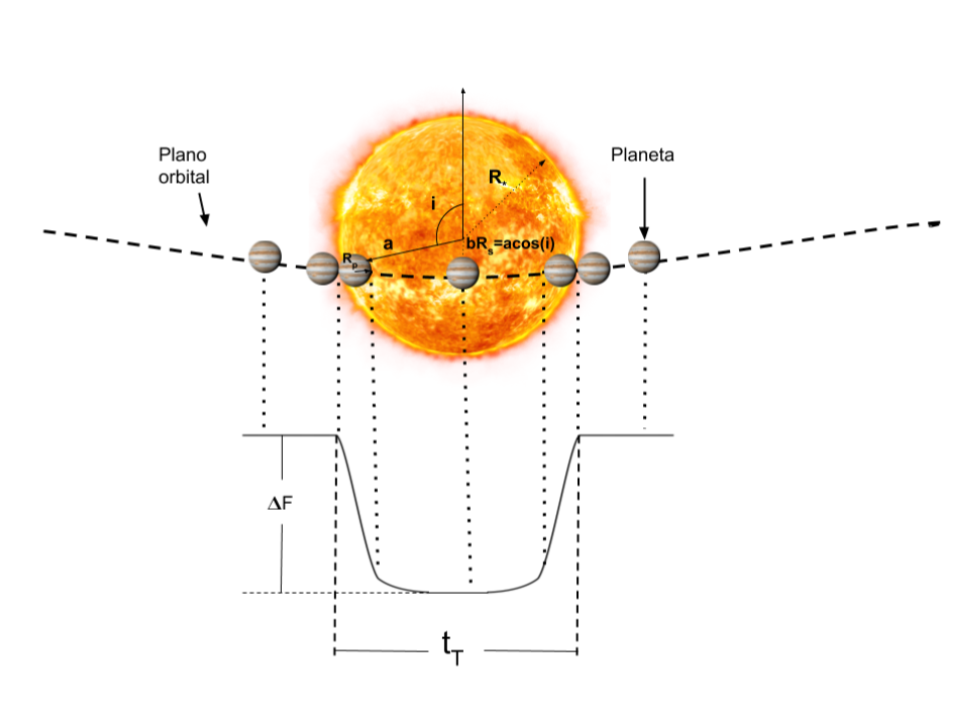
\includegraphics[max size={0.9\textwidth}{0.9\textheight}]{./figures/transito_listo.png}
   \caption{Proceso que ocurre durante un tránsito planetario. La curva en la parte inferior representa el flujo de la estrella medido por el observador, $i$ representa la inclinación de la órbita, $R_{*}$ es el radio de la estrella, $R_{p}$ el radio del planeta, $\Delta F$ es el cambio en el flujo visto por el observador, $t_{T}$ es la duración total del tránsito y $b$ el parámetro de impacto.}
    \label{fig_2_2_transito_curva}
\end{figure}
 
Utilizando la información contenida en las curvas de luz de tránsitos, podemos calcular el radio del planeta $R_{p}$ y el periodo orbital $P$, \textcolor{red}{ si se tienen múltiples observaciones simultáneas del evento; POR QUÉ?}, y si el radio de la estrella $R_{*}$ es conocido. Para los demás parámetros orbitales se necesita información complementaria de la dinámica de los cuerpos, normalmente obtenida mediante la técnica de velocidad radial. Es por este motivo que para la confirmación de un exoplaneta, este debe ser detectado por un mínimo de 2 técnicas diferentes.

\subsection*{II.1.2 Efecto del oscurecimiento del limbo en las curvas de luz}
\addcontentsline{toc}{subsection}{II.1.2 Efecto del oscurecimiento del limbo en las curvas de luz}

Las ecuaciones de la subsección anterior y sus soluciones no consideran el oscurecimiento del limbo el cual denotaremos como LD (por sus siglas en inglés). 

Es posible incorporar el efecto del LD a la descripción matemática del tránsito, incorporando un modelo en el cual el brillo de la estrella varía en función de la distancia a su centro. Esto puede provocar que la profundidad del tránsito $\Delta F$ se vea afectada, a su vez, se pierde claridad de cuando ocurre el principio/final del eclipse. En el trabajo de \cite{mandel2002analytic} se muestra la solución analítica de la forma del tránsito, e incorporan el efecto del LD utilizando 3 distintos modelos. En la figura \ref{fig_2_3_limbDarkening} podemos observar curvas de luz de tránsitos simulados a partir de las ecuaciones propuestas por \cite{mandel2002analytic}.

\begin{figure}[h!]
  \centering
    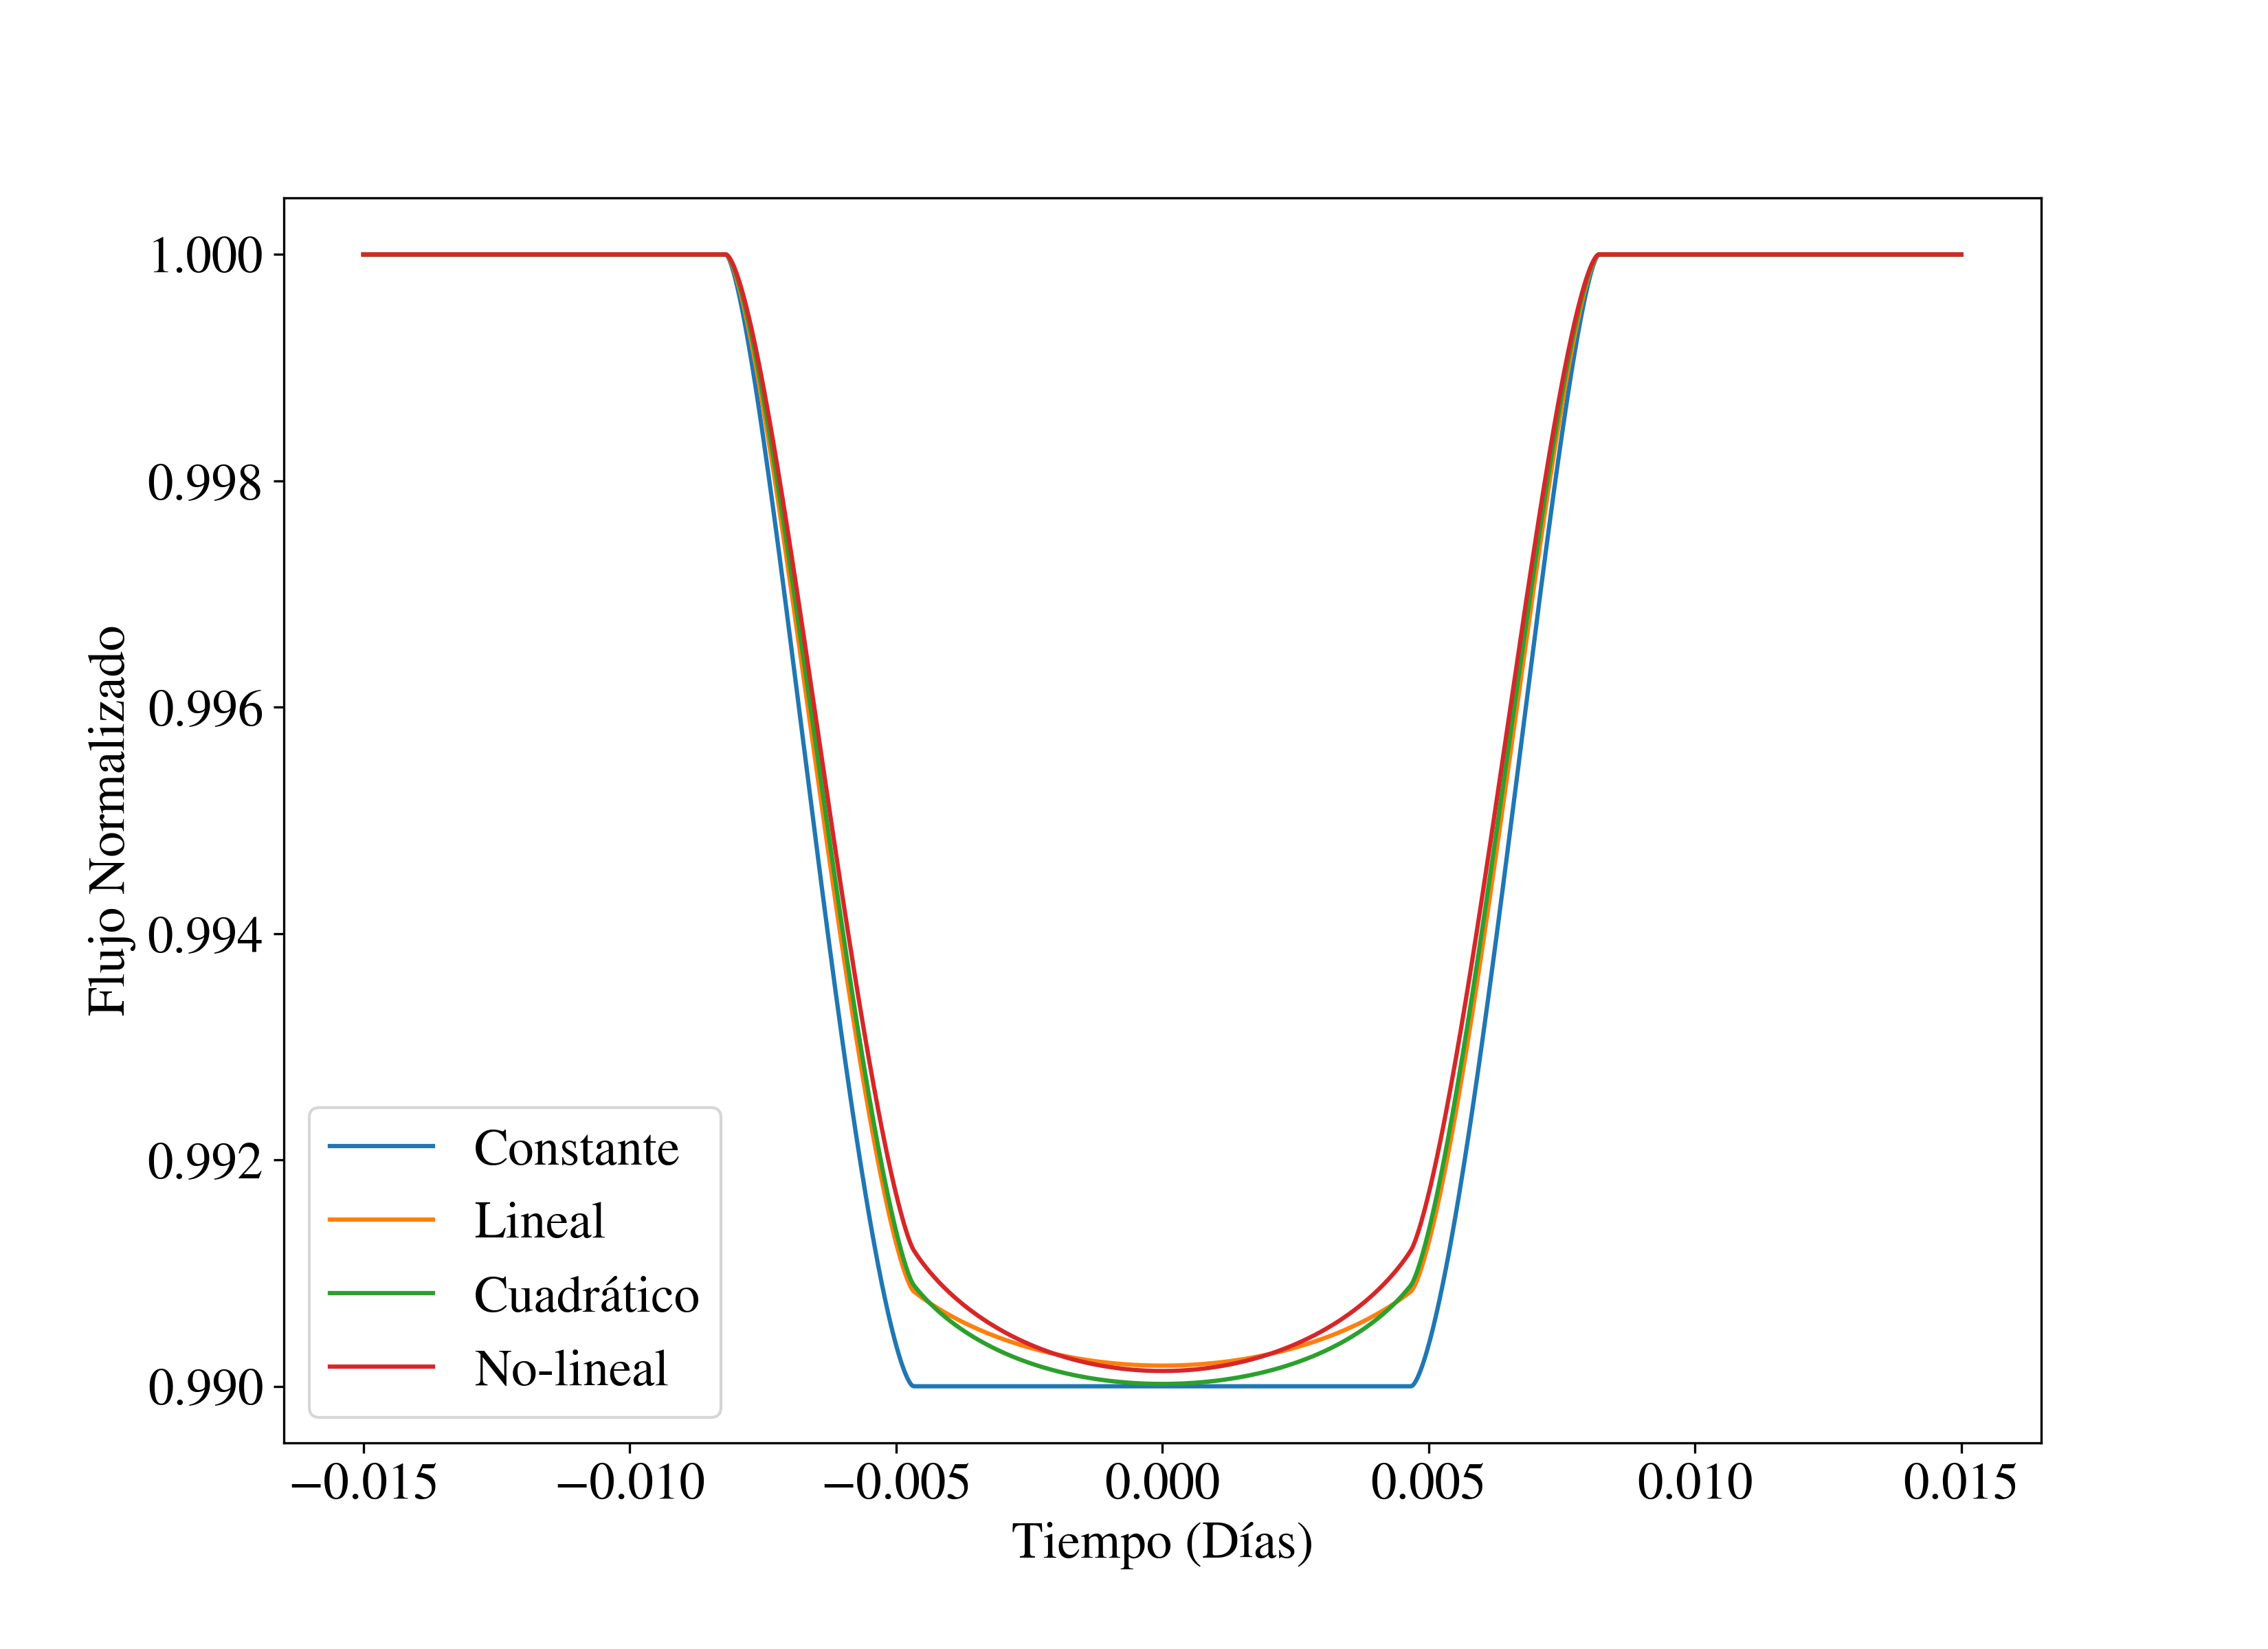
\includegraphics[max size={0.9\textwidth}{0.9\textheight}]{./figures/limbDarkening.png}
   \caption{Efecto del oscurecimiento del limbo (LD) en curvas de luz de tránsitos simulados. Se muestran 3 modelos distintos, en azul tenemos LD constante, en naranja un modelo lineal, en verde un modelo cuadrático y en rojo un modelo no-lineal. \textcolor{red}{Aquí valdría la pena agregar una curva que no considere el LD...}}
    \label{fig_2_3_limbDarkening}
\end{figure}

Para los propósitos de este trabajo, el modelo de LD que se utilice no es importante, debido a que, para la detección del tránsito, solamente buscamos detectar el cambio en el flujo $\Delta F$ independientemente de la forma de la curva de luz. El modelo de reconocimiento utilizado y descrito más adelante (véase III.6.1) es equivalente a una curva de luz con un LD constante.

\subsection*{II.1.3 Falsos positivos en la búsqueda de tránsitos}
\addcontentsline{toc}{subsection}{II.1.3 Falsos positivos en la búsqueda de tránsitos}

Los grandes proyectos como \textit{TESS} y \textit{Kepler}, observan miles, incluso cientos de miles de estrellas de manera simultánea, esto aumenta significativamente la probabilidad de encontrar sistemas planetarios, cuyo plano orbital se encuentra lo suficientemente alineado con la linea de visión ($i\sim 90^{\circ}$), para poder observar un tránsito exoplanetario (véase Fig 2.1). Por lo general, los datos recolectados por estos grandes proyectos, son preprocesados de manera automática, y se archivan las curvas de luz de interés en las cuales se observan algunas características similares a las que tendría un tránsito real. En el caso de \textit{Kepler}, la estrella se cataloga como \textit{Kepler Object of Interest (KOI)}, sin embargo, un porcentaje de estos objetos de interés no son realmente planetas. Las posibles detecciones fallidas se dividen en dos grupos: falsos positivos y falsas alarmas.

Los falsos positivos ocurren cuando tenemos curvas de luz que parecen ser producidas por un tránsito de exoplanetas pero no lo son, los dos casos más comunes son lo siguientes:

\begin{itemize}
\item \textbf{Estrellas binarias eclipsantes}: son eventos muy similares a los tránsitos, la diferencia es que una estrella es eclipsada por otra estrella compañera. En algunos casos es evidente a simple vista, que la curva de luz no tiene la forma que produciría un planeta. Sin embargo, algunas veces la caída del brillo puede ser muy similar a la producida por un tránsito exoplanetario. Estos falsos positivos son descartados después de un análisis más detallado de la curva de luz, al observar la forma y profundidad del tránsito secundario o analizando las variaciones de fase \citep{bryson2017kepler}.
\item \textbf{Binarias eclipsantes o tránsitos de fondo}: ocurren cuando ya sea un sistema binario eclipsante o un tránsito sucede en una estrella que ocupan el mismo espacio en el cielo nocturno, es decir objetos que están tan cerca en el plano del cielo que parecen ser un solo objetivo. Este fenómeno es un caso particular del primer falso positivo más común.
\end{itemize}

Algunas veces también se observan falsas alarmas, las cuales son curvas de luz con variaciones en el flujo que no son debidas a ningún tipo de tránsito. Pueden ser causadas por variabilidad estelar, condiciones atmosféricas para el caso de telescopios terrestres y/o fallas instrumentales. Por ejemplo, para el telescopio espacial \textit{Kepler} se estima que cerca del 10\% de todos los candidatos son falsos positivos \textcolor{red}{en este párrafo estás hablando de falsas alarmas no de falsos positivos, considera donde poner esta cifra} \citep{fressin2013false}.


\section*{II.2 Observación convencional de tránsitos de exoplanetas}
\addcontentsline{toc}{section}{II.2 Observación convencional de tránsitos de exoplanetas}

Los proyectos dedicados a la detección de tránsitos de exoplanetas (véase I.2), forman parte de los más exitosos proyectos en el área. Todos ellos observan estrellas utilizando prácticamente los mismos principios en cuanto a tiempos de exposición de las imágenes obtenidas, y reducción de las mismas en curvas de luz para su análisis.

Para detectar exitosamente un tránsito exoplanetario, se necesita medir con precisión el flujo proveniente de su estrella anfitriona. Por ejemplo, el tránsito de Júpiter frente a al Sol, provoca una caída en el flujo de $\sim 1\%$. Es por esto que se necesitan técnicas fotométricas para aumentar la precisión de la curva de luz. Debido a este mismo motivo, se vuelve complicado detectar planetas más pequeños desde telescopios en Tierra.

Por lo general, se utilizan tiempos de exposición de (30s - 120s), dependiendo de la magnitud de la estrella observada. Cuando el planeta es suficientemente grande, y se tiene una buena SNR (del inglés \textit{Signal to Noise Ratio}) se puede observar a simple vista el tránsito en la curva de luz, en la \textcolor{red}{Figura 2.1, debería ser 2.4} se muestra un ejemplo de una curva de luz del exoplaneta XO-3 \citep{johns2008xo} utilizando 30 segundos de exposición tomada desde el telescopio de $84~cm$ en el Observatorio Astronómico Nacional (OAN-SPM) el 21 de octubre del 2016, en la cual se puede apreciar el tránsito sin ningún post-procesamiento en la curva de luz.

\begin{figure}[h!]
  \centering
    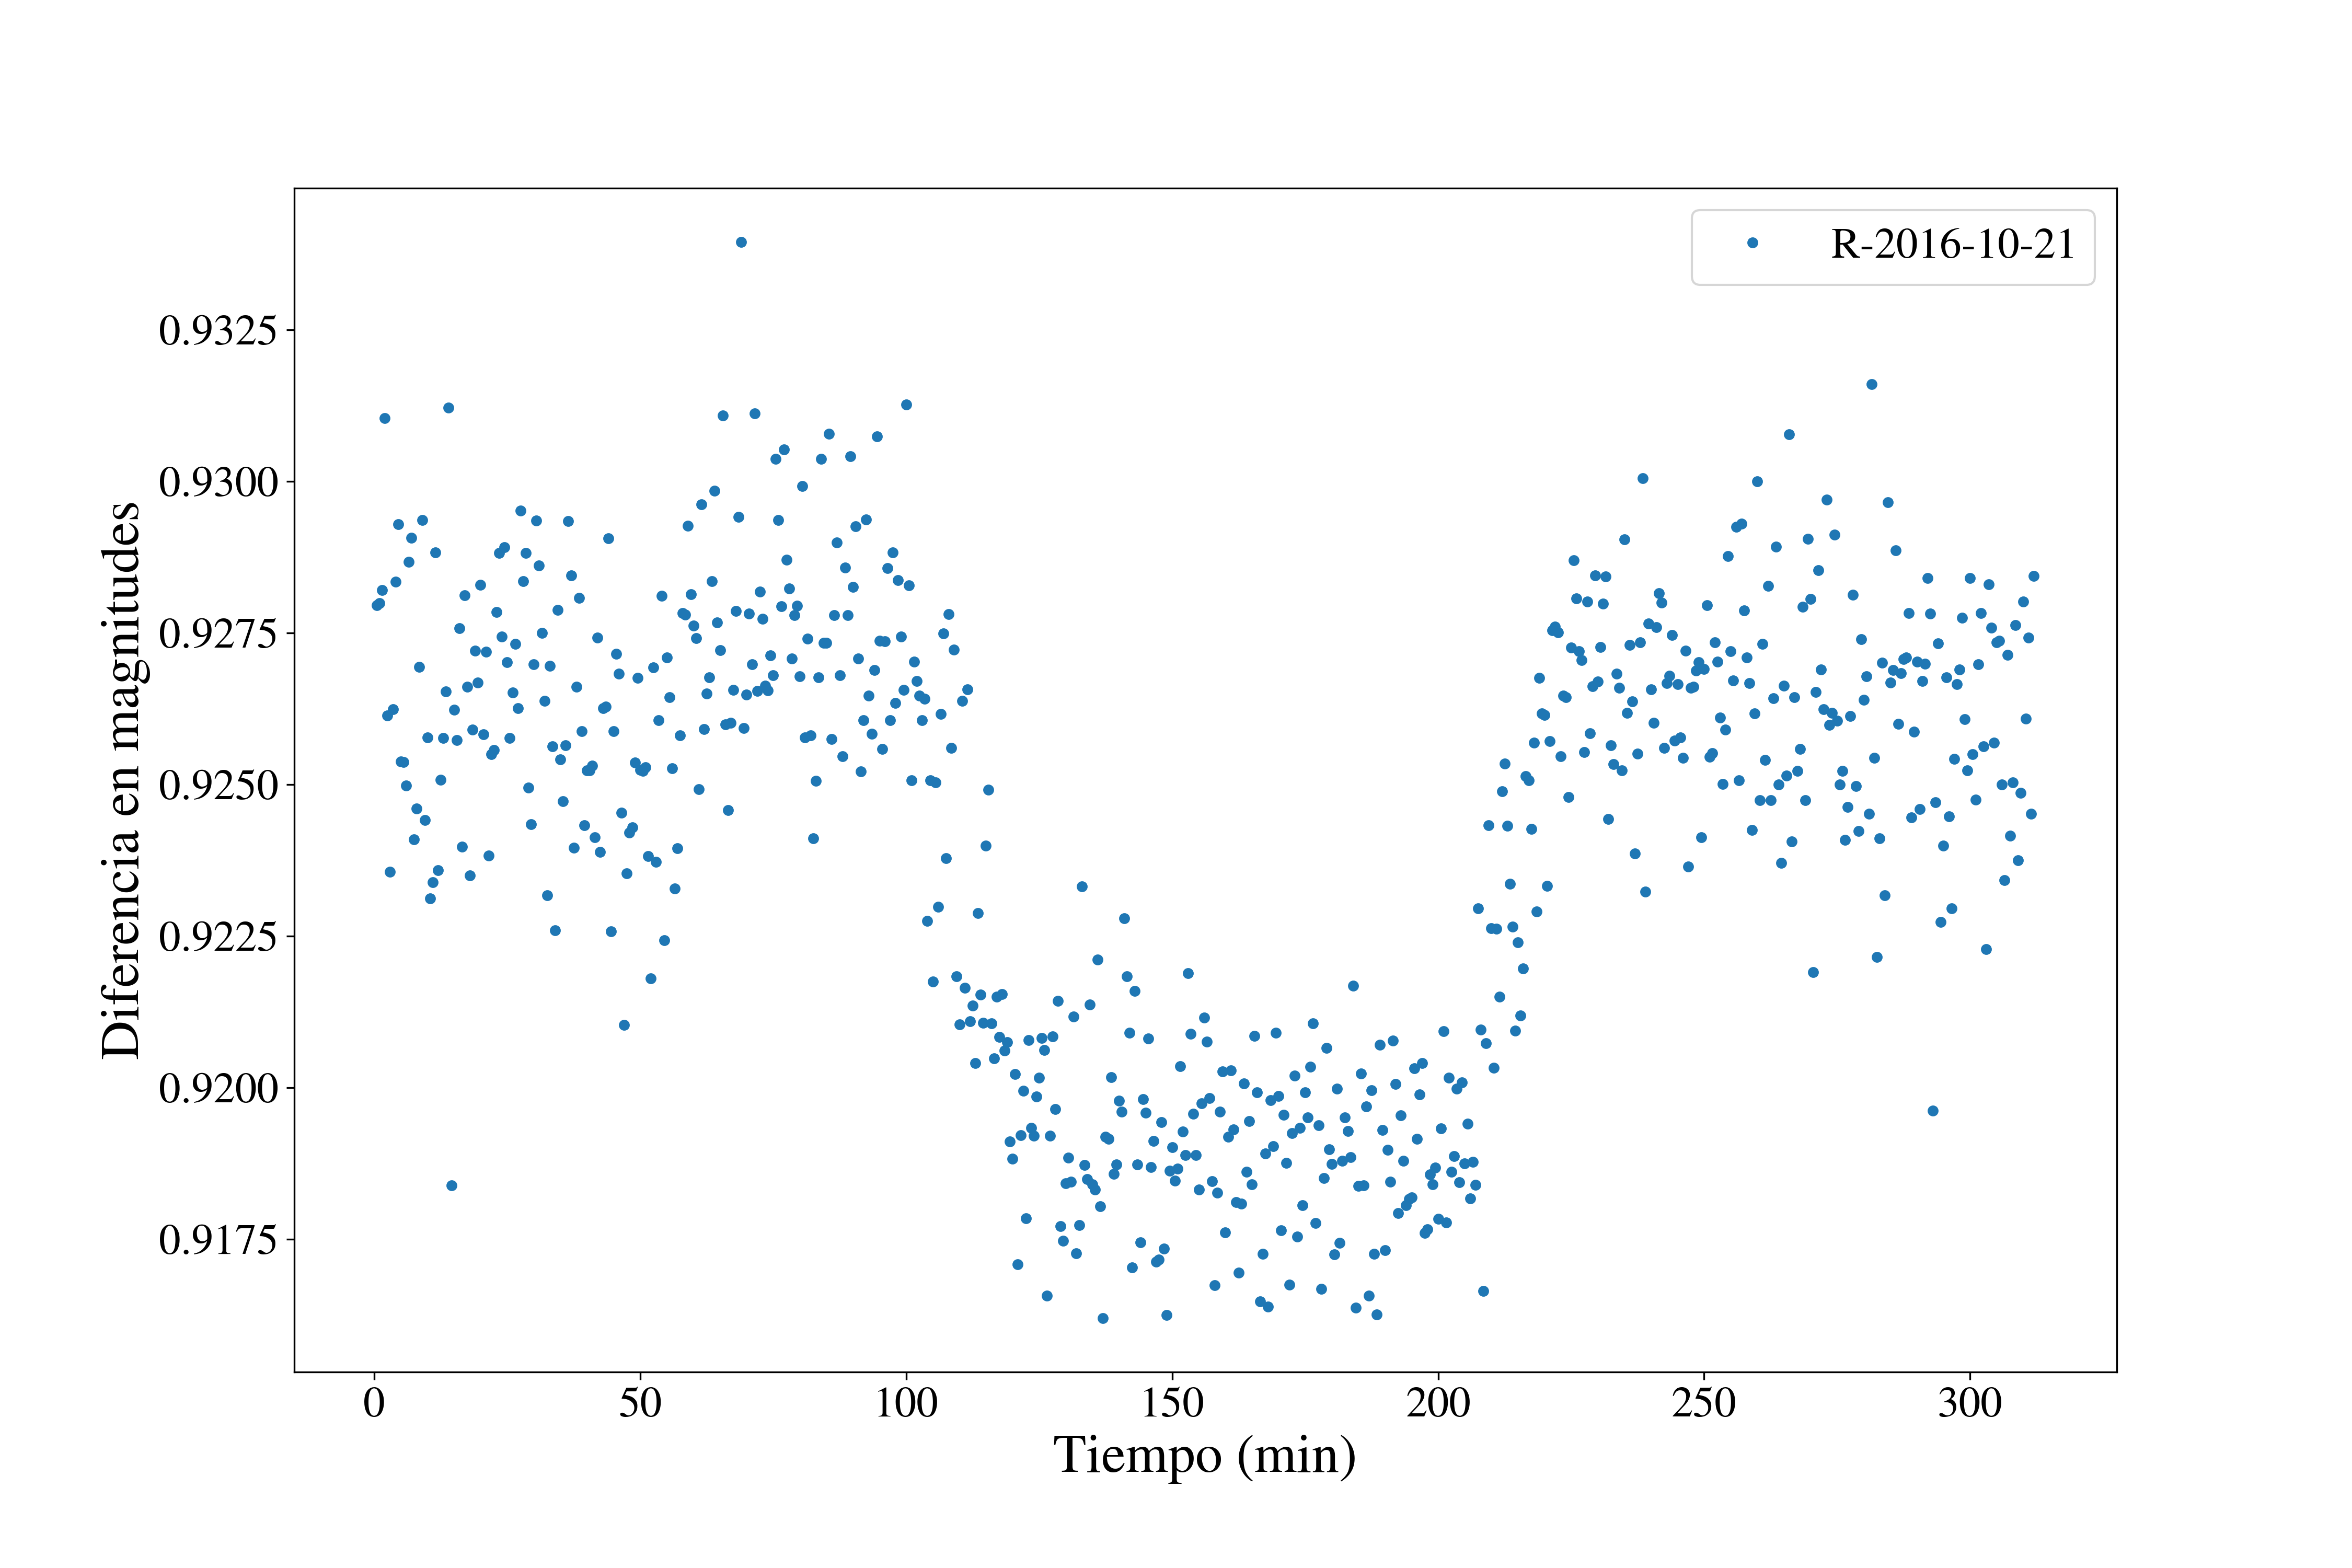
\includegraphics[max size={0.9\textwidth}{0.9\textheight}]{./figures/transitoXO3.png}
   \caption{Curva de luz de XO-3, tomada con el filtro R de Johnson en el telescopio de $84~cm$ en el Observatorio Astronómico Nacional (OAN-SPM) el 21 de octubre del 2016.}
    \label{fig_2_4_XO3}
\end{figure}

\section*{II.3 Reducción de imágenes en curvas de luz}
\addcontentsline{toc}{section}{II.3 Reducción de imágenes en curvas de luz}

Como mencionamos en la sección anterior, necesitamos medir con precisión el flujo $f_{\lambda}$ recibido de las estrellas. Es decir, medir la energía por segundo, por unidad de área, \textcolor{red}{ por unidad de longitud de onda, POR QUÉ LONGITUD DE ONDA??}:

\begin{equation}
  \displaystyle f_{\lambda}=W s^{-1}m^{-2}nm^{-1}.
\end{equation}

Para esto, utilizamos cámaras equipadas con CCD's (\textit{Couple Charge Detectors}) los cuales son un conjunto de ``chips'', generalmente de silicio muy sensibles a la luz. Cada CCD está conformado por una matriz de estos ``chips'', mejor conocidos como pixeles (para mayor detalle sobre su funcionamiento véase \cite{mortara1981evaluations}).

Estos dispositivos en combinación con grandes telescopios, nos brindan imágenes de alta calidad. Por lo general, en astronomía se utilizan CCD's monocromáticos debido a que son más sensibles y puede hacerse mejor ciencia con ellos, a diferencia de los CCD's a colores, como las cámaras comerciales para fotografía convencional.

\begin{figure}[h!]
  \centering
    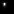
\includegraphics[scale=8]{./figures/wasp74b.png}
   \caption{Ejemplo de la imágen de una estrella estudiada en este trabajo, obtenida con una cámara rápida IXON en el telescopio de $84~cm$ en el OAN-SPM.}
    \label{fig_2_5_wasp74b}
\end{figure}

Sin embargo, las imágenes por si solas no son muy útiles cuando se quiere calcular propiedades físicas de los objetos observados, es por eso que necesitamos procesarlas para extraer información de ellas. En este trabajo, estudiamos las estrellas mediante curvas de luz, que son la medida del flujo $f_{\lambda}$ durante intervalos de tiempo regulares, las cuales se obtienen mediante un procesado denominado fotometría. Existen distintas metodologías dependiendo del objeto que se esté estudiando, en las subsecciones II.3.2 y II.3.3 se explican 2 de ellas.

\subsection*{II.3.1 Preprocesamiento de imágenes}
\addcontentsline{toc}{subsection}{II.3.1 Preprocesamiento de imágenes}

El preprocesado de las imágenes de ciencia nos ayuda a tener mejores resultados después de la fotometría, este proceso limpia las imágenes de variaciones sistemáticas, aberraciones del espejo, ruido electrónico, entre otras. Para esto, es necesario contar con imágenes de calibración comumente llamadas \textit{bias}, \textit{darks} y \textit{flats}, las cuales describiremos a continuación:

\begin{itemize}
  \item bias: estas imágenes son resultado de la lectura del CCD, sin exponer el detector a la radiación. Es decir una imágen tomada con cero segundos de exposición. Estas imágenes contienen información sobre el ruido electrónico y el ruido de lectura del CCD. 
  \item darks: estas imágenes resultan de integrar el CCD \textit{t} segundos de integración, pero de igual manera que los \textit{bias}, sin exponer el detector a ningún tipo de radiación externa. Se recomienda que los \textit{darks} y las imágenes de ciencia tengan el mismo tiempo de exposición \textit{t}.
  \item flats: estas imágenes resultan de exponer todo el detector a una fuente brillante uniforme. Se busca que todo el detector este sometido a un nivel de radiación similar al objetivo que se va a estudiar. Esto nos ayuda a detectar  y corregir las irregularidades en las imágenes por el detector mismo, la óptica del telescopio, polvo, etc. Existen diversas maneras de tomar \textit{flats}, para más detalle véase \cite{chromey1996special}.
\end{itemize}

Es necesario contar con un conjunto de imágenes de calibración, de 20 a 40, para cada una de las mencionadas anteriormente. Para el tratamiento matemático con estas imágenes, denotaremos a los \textit{bias}, \textit{darks} y \textit{flats} como $B_{t}(x,y)$, $D_{t}(x,y)$ y $F_{t}(x,y)$ respectivamente.

El primer paso en el preprocesamiento es obtener las "\textit{master images}" de cada conjunto. El \textit{bias master} $B_{master}(x,y)$ se obtiene al calcular la mediana por pixel de todo el conjunto de \textit{bias}

\begin{equation}
  \displaystyle B_{master}(x,y) = \mbox{Mdn} \left[ B_{t}(x,y) \right].
\end{equation}

Para calcular el \textit{dark master} $D_{master}(x,y)$, restamos el \textit{bias master} al conjunto de \textit{darks} y se calcula la mediana del resultado:

\begin{equation}
  \displaystyle D_{master}(x,y) = \mbox{Mdn} \left[ D_{t}(x,y) - B_{master}(x,y)\right].
\end{equation}

Para calcular el \textit{flat master} $F_{master}(x,y)$, primero restamos el \textit{bias master} al conjunto de \textit{flats} y normalizamos a 1 el resultado:

\begin{equation}
  \displaystyle F^{norm}_{t}(x,y) = \mbox{Norm} \left[ F_{t}(x,y) - B_{master}(x,y)\right],
\end{equation}

donde $\mbox{Norm}$ representa:

\begin{equation}
  \displaystyle \mbox{Norm}\left[I_{t}(x,y)\right] =  \dfrac{I_{t}(x,y)}{\dfrac{1}{m*n} \sum_{x=0}^{m}\sum_{y=0}^{n} I_{t}(x,y)}.
\end{equation}

Después, calculamos la mediana de $F^{norm}_{t}(x,y)$ y normalizamos nuevamente para obtener $F_{master}(x,y)$:

\begin{equation}
  \displaystyle F_{master}(x,y) = \mbox{Norm} \left[ \mbox{Mdn} \left( F^{norm}_{t}(x,y)\right)\right].
\end{equation}

Finalmente, utilizamos estas \textit{master images} para limpiar las imágenes de ciencia $O_{t}(x,y)$:

\begin{equation}
  \displaystyle R_{t}(x,y) = \dfrac{O_{t}(x,y) - B_{master}(x,y) - D_{master}(x,y)}{F_{master}(x,y)}.
\end{equation}

\subsection*{II.3.2 Fotometría rápida}
\addcontentsline{toc}{subsection}{II.3.2 Fotometría rápida}

La fotometría se encarga de integrar el flujo $f_{\lambda}$ medido con ayuda del CCD. Con la imagen de una estrella como la que se muestra en la Figura 2.2, se puede obtener una curva de luz mediante la fotometría rápida. Este proceso se realiza tanto como para curvas de luz, como para espectroscopía.

Cada pixel en la imagen tiene asociado un valor comunmente denominado como ``cuentas'', este valor representa el número de electrones producidos en ese pixel durante el proceso de captura de fotones. Un CCD ideal, es uno que por cada fotón produce un electrón, los CCD's de la actualidad están cerca de este límite.

La fotometría rápida consiste en sumar las ``cuentas'' de cada pixel ($x_{i},y_{i}$), de $R_{t}(x,y) $, donde $ i $ va de 1 hasta $ N $, donde $ N $ es el número de pixeles en cada eje de la imagen ciencia  y $ t $ es el número de imágenes. En este caso consideraremos el caso con imágenes simétricas, donde el número de pixeles en el eje x $(N_{x})$, y en el eje y $(N_{y})$ son iguales $N_{x}=N_{y}=N$. 

\begin{equation}
  \displaystyle F_{t} = \sum_{x_{i}}^{N} \sum_{y_{i}}^{N} R_{t}(x_{i},y_{i}),\hspace{1cm}i=1,...,N;
\end{equation}

La integración de cada imagen produce un solo valor $F_{t}$ en la curva de luz \citep{romanishin2006introduction}. Por ejemplo, la \textcolor{red}{Figura 2.1, COrregir esta referencia} fue obtenida mediante la fotometría de 624 imágenes de una región de 7x7 pixeles. Este procesado de las imágenes puede realizarse utilizando distintas metodologías. Como su nombre lo indica, la fotometría rápida toma poco tiempo generar la curva de luz y es muy útil para análisis in sitú, sin embargo, no permite observar variaciones pequeñas de flujo, púes regularmente el ruido en las imágenes es suficientemente grande para enmascarar dicha señal. En este trabajo, las curvas de luz fueron obtenidas utilizando la metodología de fotometría de apertura diferencial.

\subsection*{II.3.1 Fotometría de apertura}
\addcontentsline{toc}{subsection}{II.3.1 Fotometría de apertura}

Con el fin de mejorar la SNR en la curva de luz resultante de la fotometría, este proceso se mejora realizando lo que se conoce como fotometría de apertura, lo cual consiste en utilizar aperturas circulares para integrar el flujo de la estrella, y además se resta la contribución debido al cielo \textcolor{red}{Aunque en alta cadencia el Cielo prácticamente no contribuye}.

Primeramente definimos 2 máscaras circulares centradas en las coordenadas $(x_{c},y_{c})$ del centroide $ C_{t} $ de la estrella. El anillo formado por los círculos azules de la \textcolor{red}{Figura 2.3, debe ser \ref{fig_2_6_aperturas}},  se utiliza para restar la contribución del flujo debido al cielo $(S_{t})$, siendo $D_{t}$ el círculo exterior y $A_{t}$ el interior. La apertura de medición $M_{t}$ mostrada con un círculo rojo en la Figura 2.3 contiene información tanto de la estrella como del cielo $(F_{t}+S_{t})$ con $F_{t}$ el flujo de la estrella, de la imagen $t$.


\begin{figure}[h!]
  \centering
    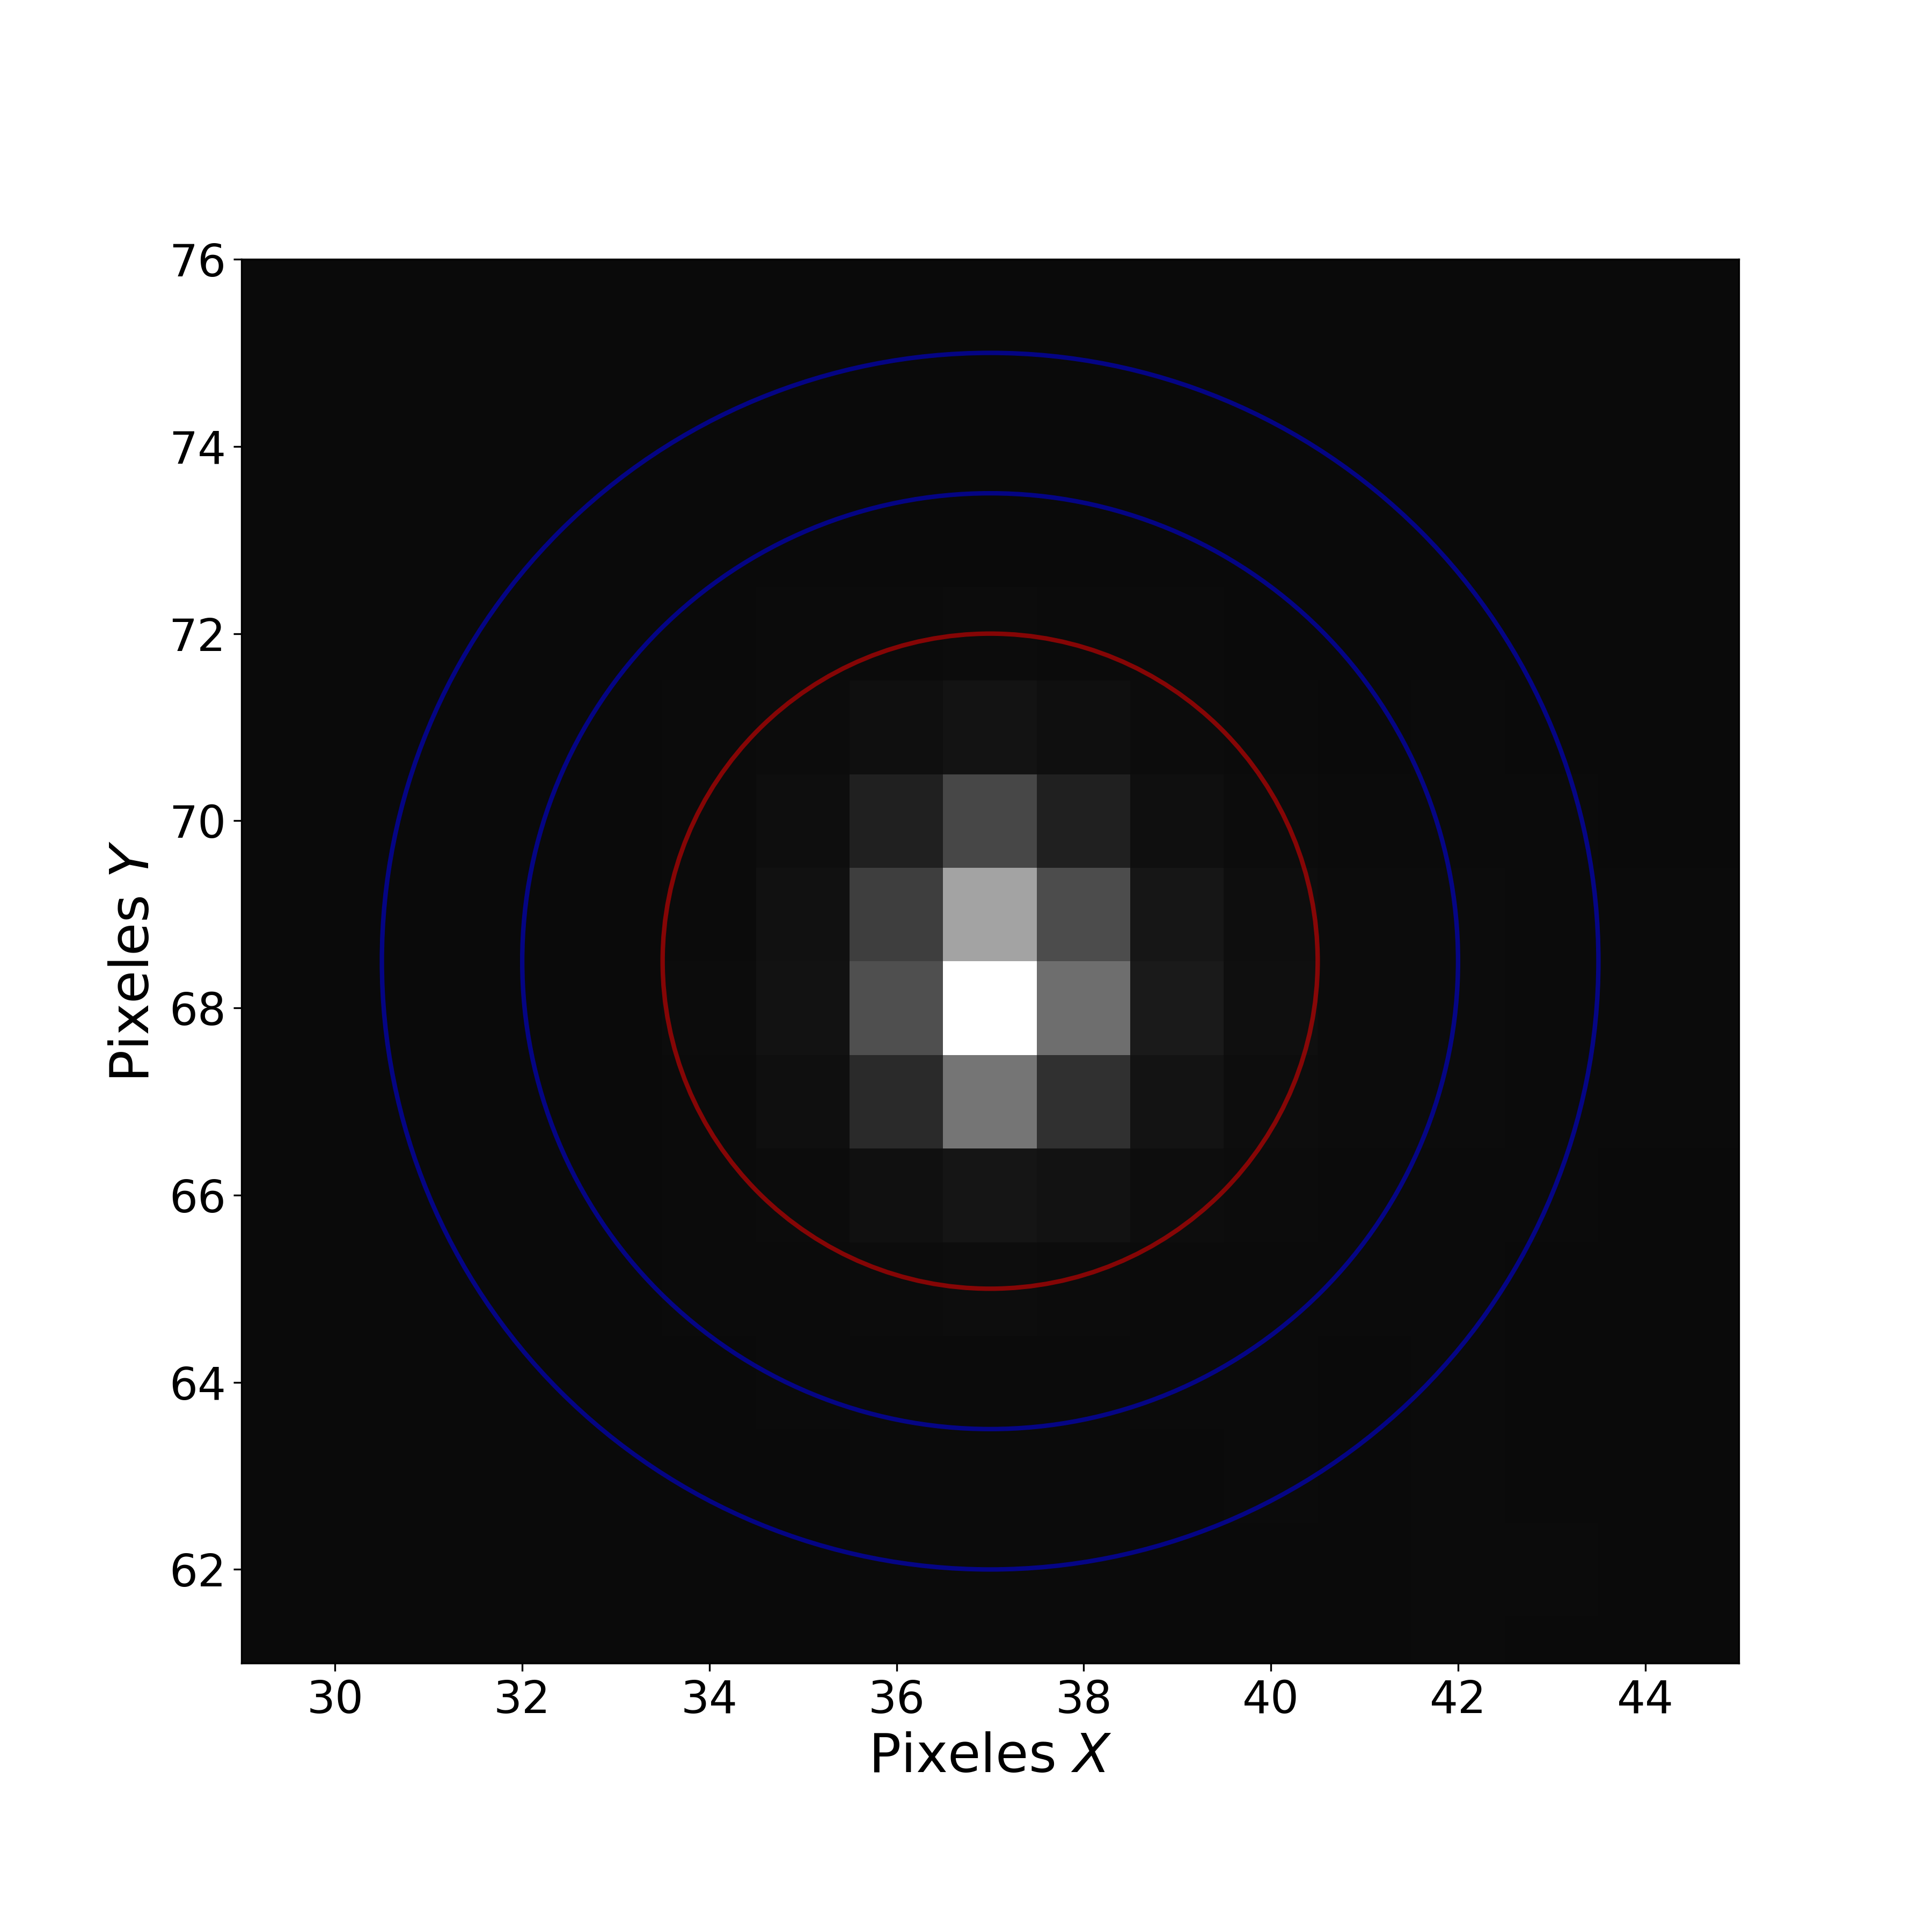
\includegraphics[max size={0.7\textwidth}{0.7\textheight}]{./figures/aperturas.png}
   \caption{Ejemplo de aperturas circulares para realizar fotometría de HAT-P-37B. El anillo formado por las circunferencias en azul se utiliza para calcular la contribución del flujo debido al cielo.\textcolor{red}{usar colores de mejor contraste para el anillo y etiquetar/resaltar las áreas correspondientes}}
    \label{fig_2_6_aperturas}
\end{figure}


Denotaremos el área entre $D_{t}$ y $A_{t}$ como $Area_{D_{t}-A_{t}}$, esta área en conjunto con $S_{t}$ se puede calcular la contribución del flujo debido al cielo por unidad de área $S^{Area}_{t}$.

\begin{equation}
  \displaystyle S^{Area}_{t} = \dfrac{S_{t}}{Area_{D_{t}-A_{t}}};
\end{equation}

El brillo del cielo por unidad de área $S^{Area}_{t}$ multiplicado por el área de $M_{t}$ denotada como $Area_{M_{t}}$	nos da la contribución del cielo dentro de $M_{t}$, es decir \textcolor{red}{esta ecuación no está clara, contiene el término $F_t$ dentro y no decribe bien el proceso, que debe ser así... se obtiene la mediana o la media del flujo del área del anillo para obtener el el valor por pixel, que luego se multiplica por el área del círculo central para obtener la contribución del cielo... Tienes que definir cada uno de los términos con palabras y en la figura}:

\begin{equation}
  \displaystyle F_{t} = F_{t} + S_{t} - \left( S^{Area}_{t}\times Area_{M_{t}}\right);
\end{equation}

Con esta metodología podemos obtener $F_{t}$ libre de contribución del cielo. Este proceso se repite para las $t$ imágenes. Si existe movimiento de la estrella debido a perturbaciones atmosféricas, o mal guiado, el centroide $ C_{t} $ se recalcula en cada imágen.


\subsection*{II.3.2 Fotometría diferencial}
\addcontentsline{toc}{subsection}{II.3.2 Fotometría diferencial}

Si en el campo de observación hay $ N $ estrellas, denotaremos la curva de luz de ellas como $F^{i}$ con $i=1,...,N$. La curva de luz de una estrella por fotometría diferencial $F^{i}_{Diff}$ se calcula utilizando $F^{i}$ y el flujo de una estrella compañera $F^{j}$, ambas obtenidas mediante fotometría de apertura. 

\begin{equation}
  \displaystyle F^{i}_{Diff}=\dfrac{F^{i}}{F^{j}};
\end{equation}

Idealmente, estas estrellas deben tener una magnitud similar $(\pm 10 \%)$ y estar cerca de una de otra ($<3$ arcmin) para que la contribución debido a la atmósfera sea comparable.


\begin{figure} [H]
  \centering
    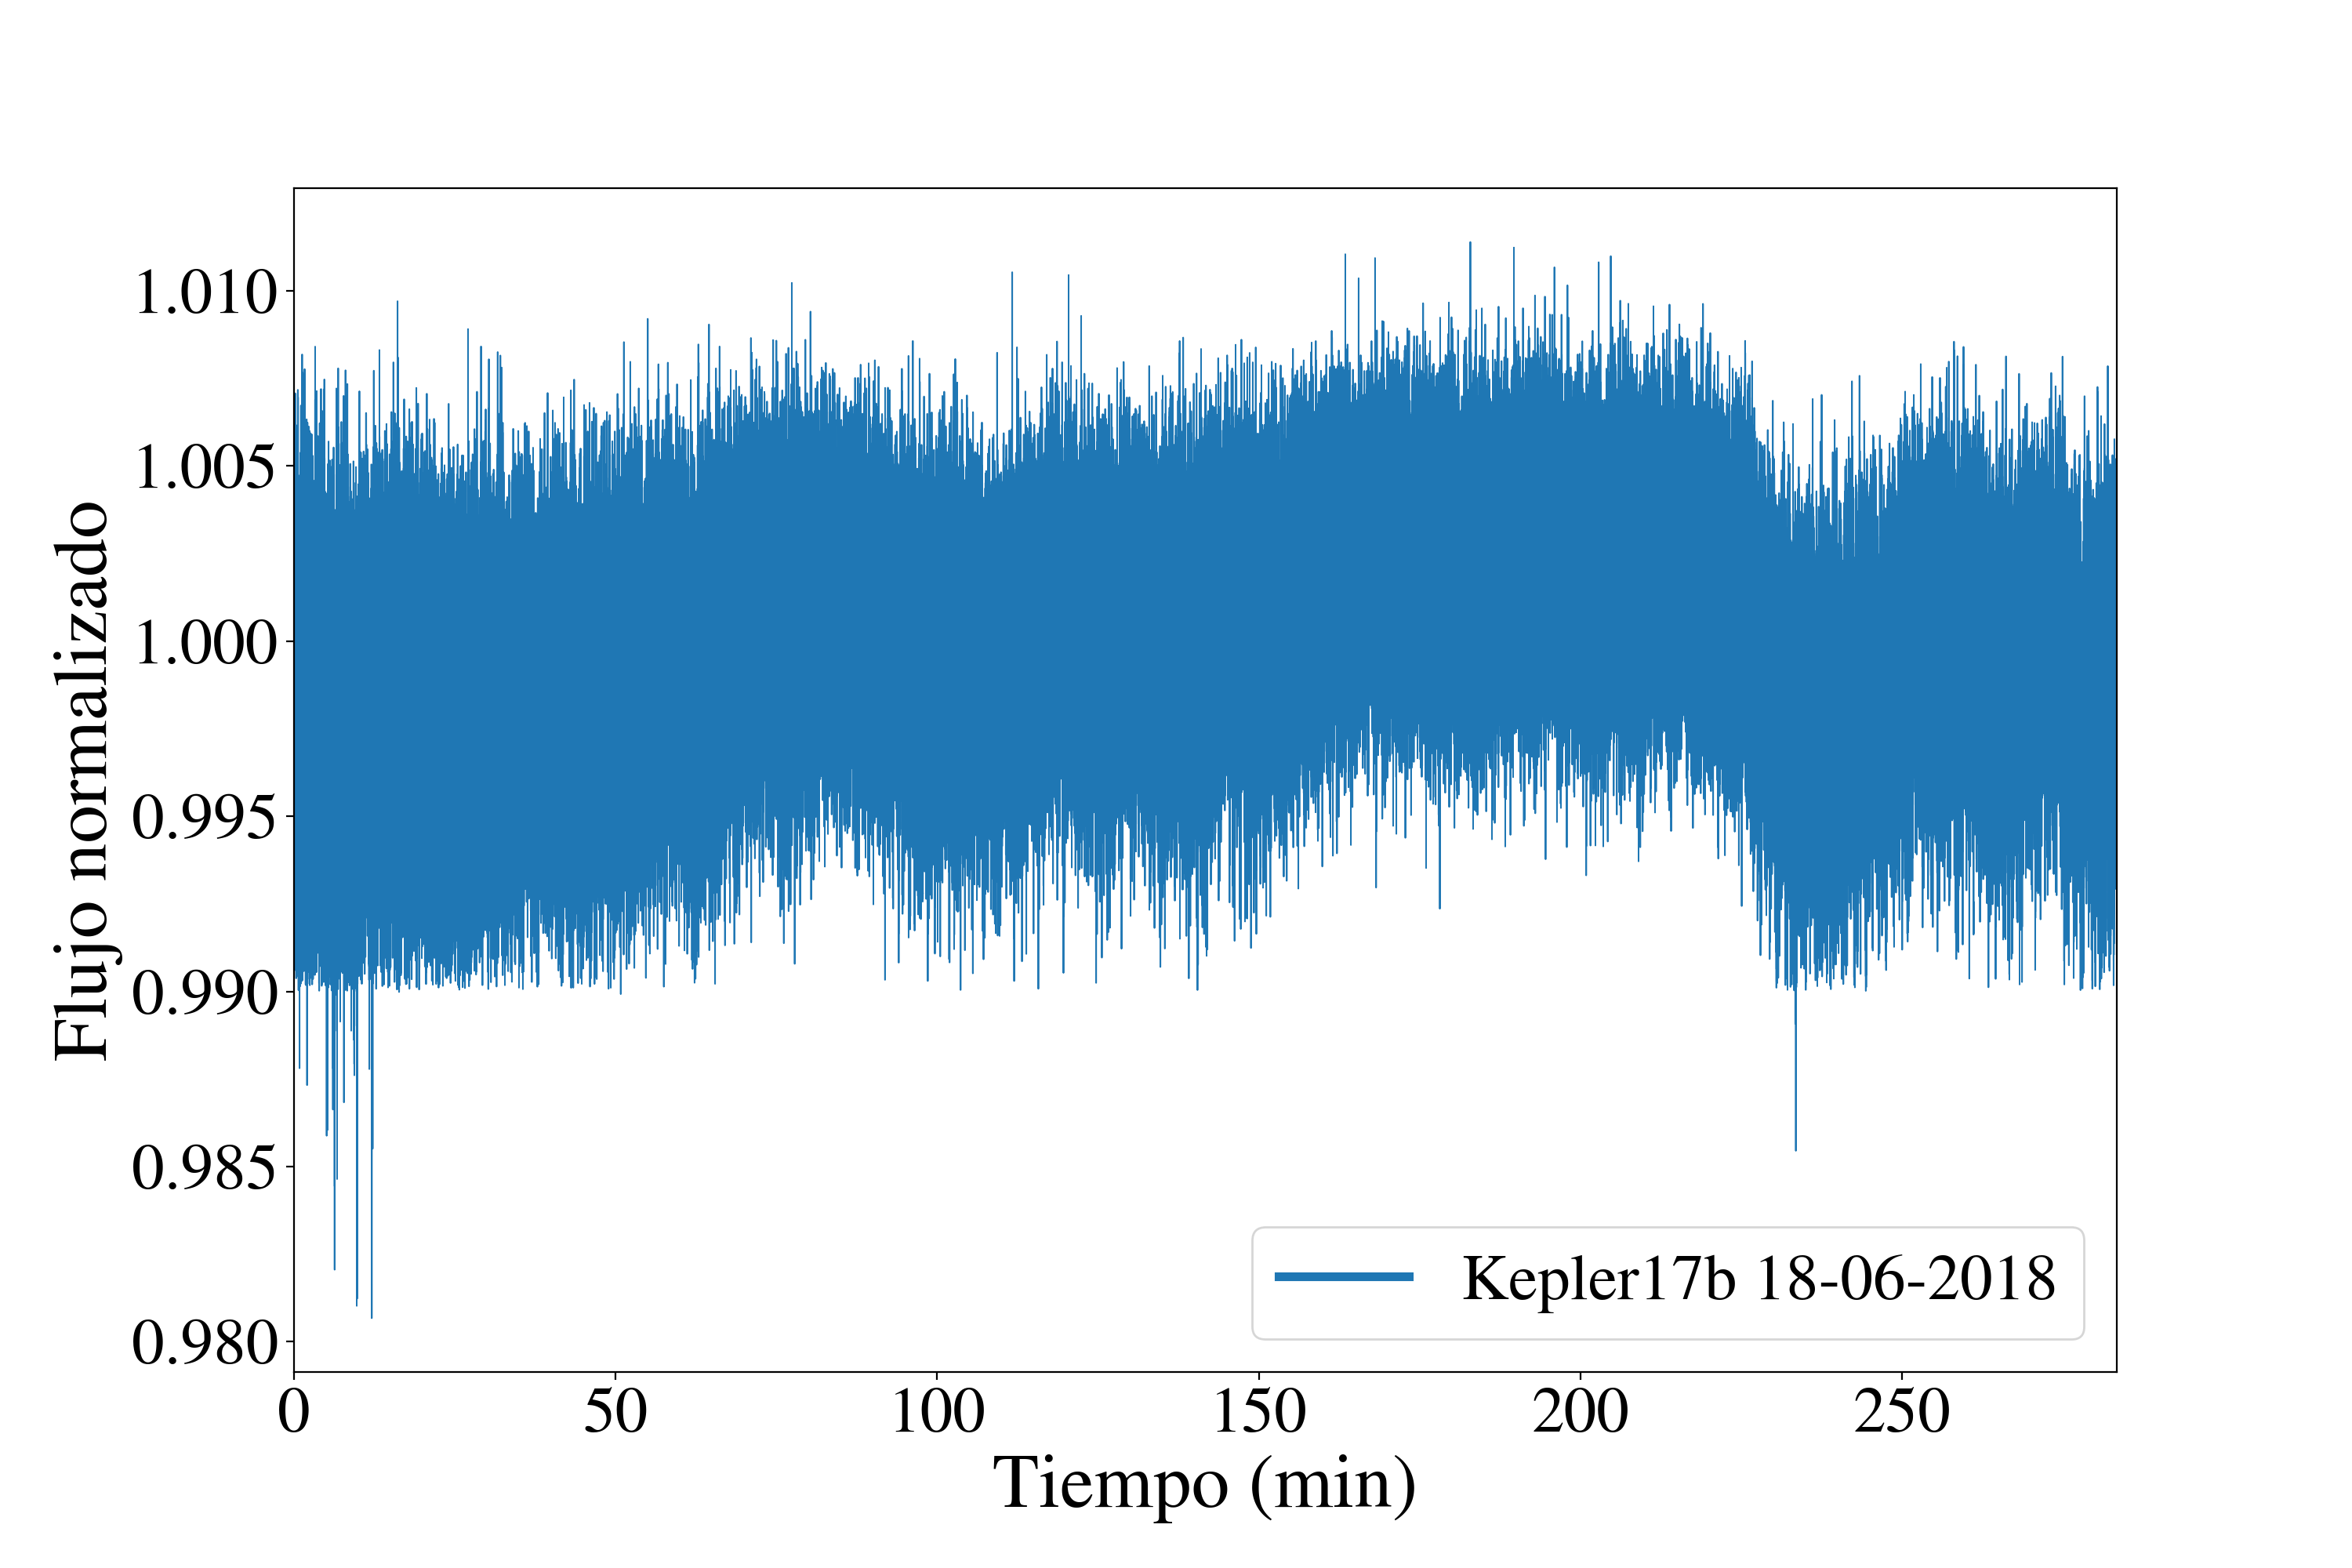
\includegraphics[max size={1\textwidth}{0.4\textheight}]{./figures/fotometria_apertura.png}
   \caption{Curva de luz de alta cadencia de Kepler17b obtenida mediante fotometría de apertura. La observación de Kepler17b se realizó en el sitio 2 de TAOS II, utilizando una cámara \textit{Zyla} de Andor. Esta curva de luz se obtuvo utilizando APPHi véase (sección III.4.1). }
    \label{fig_2_7_foto_apertura}
\end{figure}

\begin{figure}[H]
  \centering
    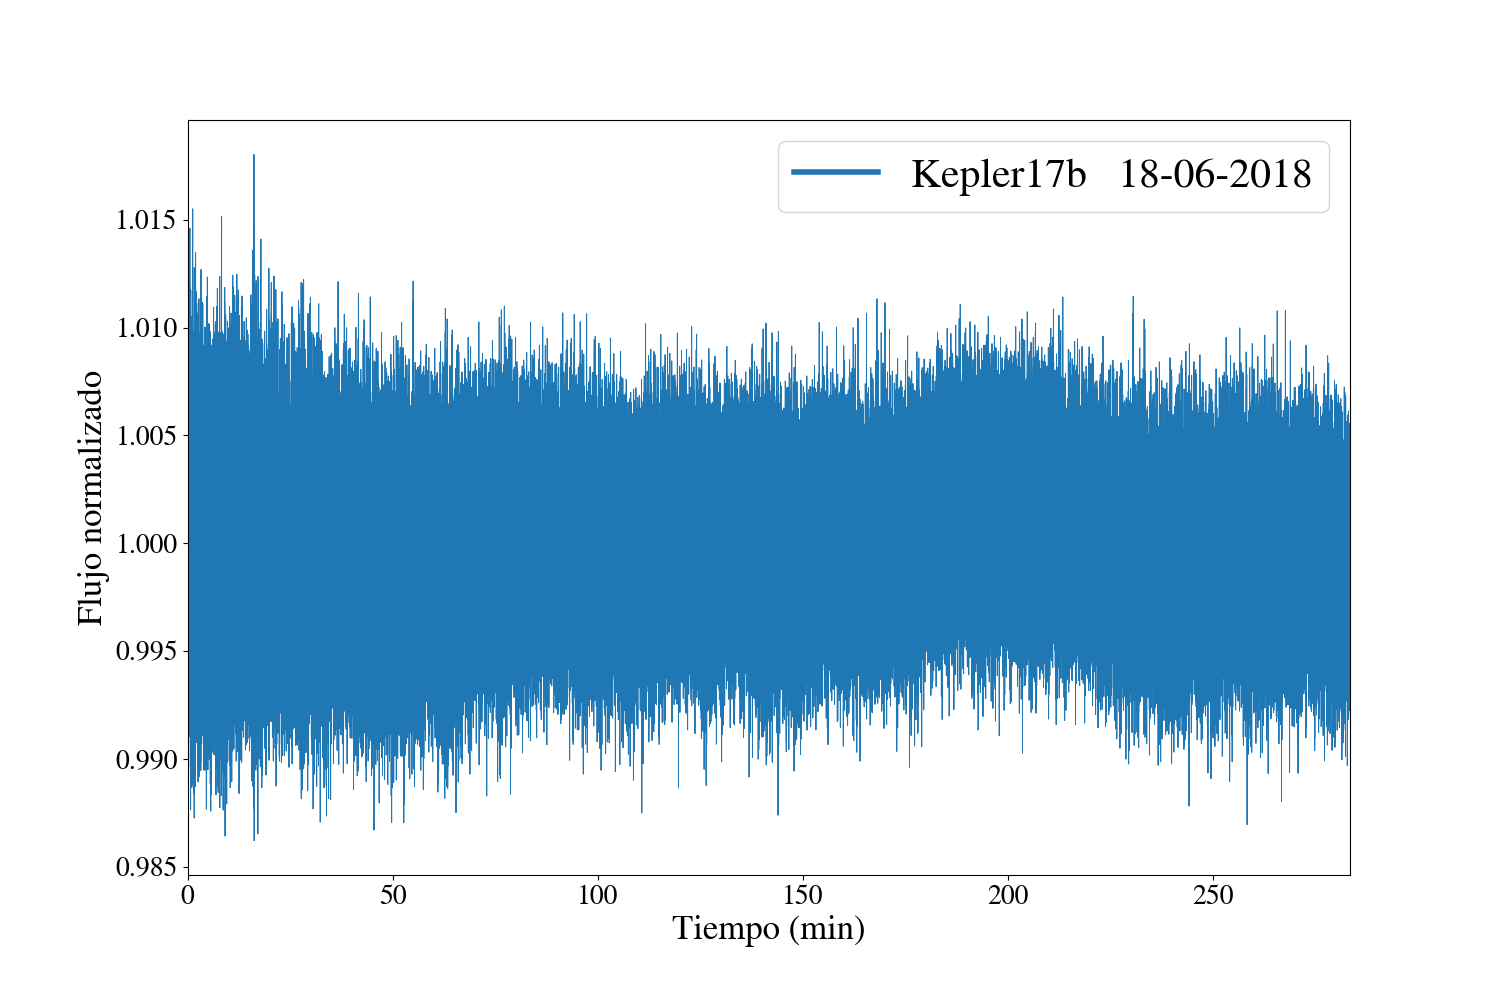
\includegraphics[max size={1\textwidth}{0.4\textheight}]{./figures/fotometria_diferencial.png}
   \caption{Curva de luz de alta cadencia de Kepler17b obtenida mediante fotometría diferencial. La observación de Kepler17b se realizó en el sitio 2 de TAOS II, utilizando una cámara \textit{Zyla} de Andor. Esta curva de luz se obtuvo utilizando APPHi véase (sección III.4.1).}
    \label{fig_2_8_foto_diferencial}
\end{figure}


\section*{II.4 Análisis de ruido en series de tiempo}
\addcontentsline{toc}{section}{II.4 Análisis de ruido en series de tiempo}

El análisis de las series de tiempo se basa en suponer que el flujo observado en la curva de luz de la estrella que se está estudiando $(F^{obs}_{t})$, está  compuesto a partir de la contribución de distintos fenómenos:

\begin{equation}
  \displaystyle F^{obs}_{t}=F_{t}\times R_{t};
\end{equation}

\noindent donde $F^\_{t}$ es el flujo real de la estrella, sin ningún tipo de contribución debido a la atmósfera o el instrumento de medición. Todas estas contribuciones que añaden ruido al flujo observado están representadas por $R_{t}$. A su vez, $R_{t}$ está conformado por ruido de alta o baja frecuencia. 

Las componentes de baja frecuencia se conocen como ``tendencias'', se define como un cambio suave del flujo en la curva de luz a largo plazo que afecta a todas las estrellas del campo en forma similar. Generalmente provocadas por condiciones climáticas como la masa de aire, la cual cambia lentamente en unas horas de observación. Otras variables climáticas como densidad del aire, presión y cantidad de agua en la atmósfera cambian más rápidamente, en escalas de tiempo de minutos. Las componentes de alta frecuencia se deben principalmente a ruido electrónico al momento de la lectura del CCD y a la aberraciones del frente de onda causados por la atm\'osfera. Tiempos de exposición largos $(T_{exp} \sim 100 s)$ disminuyen la contribución del ruido de lectura, sin embargo en este trabajo nos enfocaremos en estudiar curvas de luz de alta cadencia $(T_{exp} < 1 s)$, por lo tanto, la imagen se lee mas veces por unidad de tiempo, lo cual incrementa en esa misma medida el ruido electr\'onico \textcolor{red}{(aquí puede quedar nuestro paper de efectos atmosféricos, no tardan en publicarlo)}.

Estos fenómenos representados en $R_{t}$, afectan la curva de luz creando un ruido aleatorio, el cual puede tener diferentes distribuciones estadísticas como Gaussiana o de Poisson o una convolución de estas distribuciones \cite{luisier2010image}.

Entender el comportamiento de cada componente es importante cuando se desea realizar un análisis numérico, debido a que si se desea simular una curva de luz, esta debe contener la suma de las distintas componentes que conforman una señal real (véase sección II.2). Para el caso de las curvas de luz, estas componentes son catalogadas como tipos de ruido. Como se mencionó anteriormente, el ruido en las curvas de luz, cambia de manera significativa dependiendo de la cadencia de adquisición.

Los tipos de ruido que están presentes en todas las curvas de luz, son el ruido instrumental, el producido por la masa de aire y el causado por las condiciones climáticas. Estos tipos de ruido afectan por igual a las imágenes de alta y baja cadencia, y el tratamiento estadístico utilizado para eliminarlo es el mismo en ambos tipos de curvas. Sin embargo, el ruido en las curvas de luz de alta cadencia, es mucho mas notable que en las de baja cadencia. Esto se debe a que el tiempo de exposición es corto, por lo tanto se captan menos fotones provenientes de la estrella, y la magnitud del ruido de lectura puede llegar a ser comparable con la de la estrella. Esto provoca que la señal de un tránsito en la estrella $F^{t}$  se vea ocultada por el ruido $R_{t}$ \cite{pont2006effect}. Para cuantificar la contribución del ruido, calculamos el coeficiente de señal a ruido (SNR):

\begin{equation}
  \displaystyle SNR=\dfrac{\bar{F}^{obs}_{t}}{\sigma};
\end{equation}

\noindent donde $\bar{F}^{obs}_{t}$ es la media aritmética de la curva de luz y $\sigma$ su desviación estándar.

Por otra parte, analizar el espectro de frecuencias de la serie de tiempo, nos puede dar información sobre las distintas componentes de ruido como veremos a continuación.

\section*{II.5 Transformada de Fourier para estudiar series de tiempo}
\addcontentsline{toc}{section}{II.5 Transformada de Fourier para estudiar tiempo y frecuencia}

Dentro del estudio de las series de tiempo, una herramienta matemática fundamental es la transformada de Fourier (FT), definida de manera analítica como:

\begin{equation}
  \displaystyle \mathcal{F}(\omega )=\frac{1}{\sqrt{2\pi}}\int_{-\infty}^{\infty} f(t)e^{i\omega t}dt;
\end{equation}

\noindent donde $\mathcal{F}(\omega )$ es la transformada de Fourier de $f(t)$. Sin embargo, al trabajar con series de tiempo numéricas haremos uso de la transformada de Fourier discreta (DFT):  

\begin{equation}
  \displaystyle \mathcal{F}_{\omega}= \sum_{n=0}^{N-1} F_{t}e^{-\dfrac{i2\pi}{N}\omega t};
\end{equation}

\noindent de la ec. 2.13 podemos observar que es necesario realizar $N$ multiplicaciones y $N$ sumas, lo que resulta en $N^{2}$ operaciones. El método más usual de calcular una transformada de Fourier Discreta es utilizar el algoritmo conocido como \textit{Fast Fourier Transform} (FFT). Como su nombre lo indica, es una manera de calcular la transformada más eficientemente, lo cual es útil cuando analizamos una gran cantidad de datos y/o $N$ es grande. En la FFT se reduce el número de operaciones a $Nlog_{2}N$ \citep{cooley1965algorithm}. 

Esta transformada integral, nos ayuda a convertir una serie de tiempo $F_{t}$, a una serie de frecuencias $\mathcal{F}_{\omega}$, también llamado \textit{espectro de frecuencias}. Las variaciones sistemáticas en la serie de tiempo $F_{t}$ provocan ``picos'' en el espectro de frecuencias, identificar estas componentes de frecuencia nos ayuda a visualizar las diferentes contribuciones de ruido a la curva de luz.

\begin{figure}
  \centering
    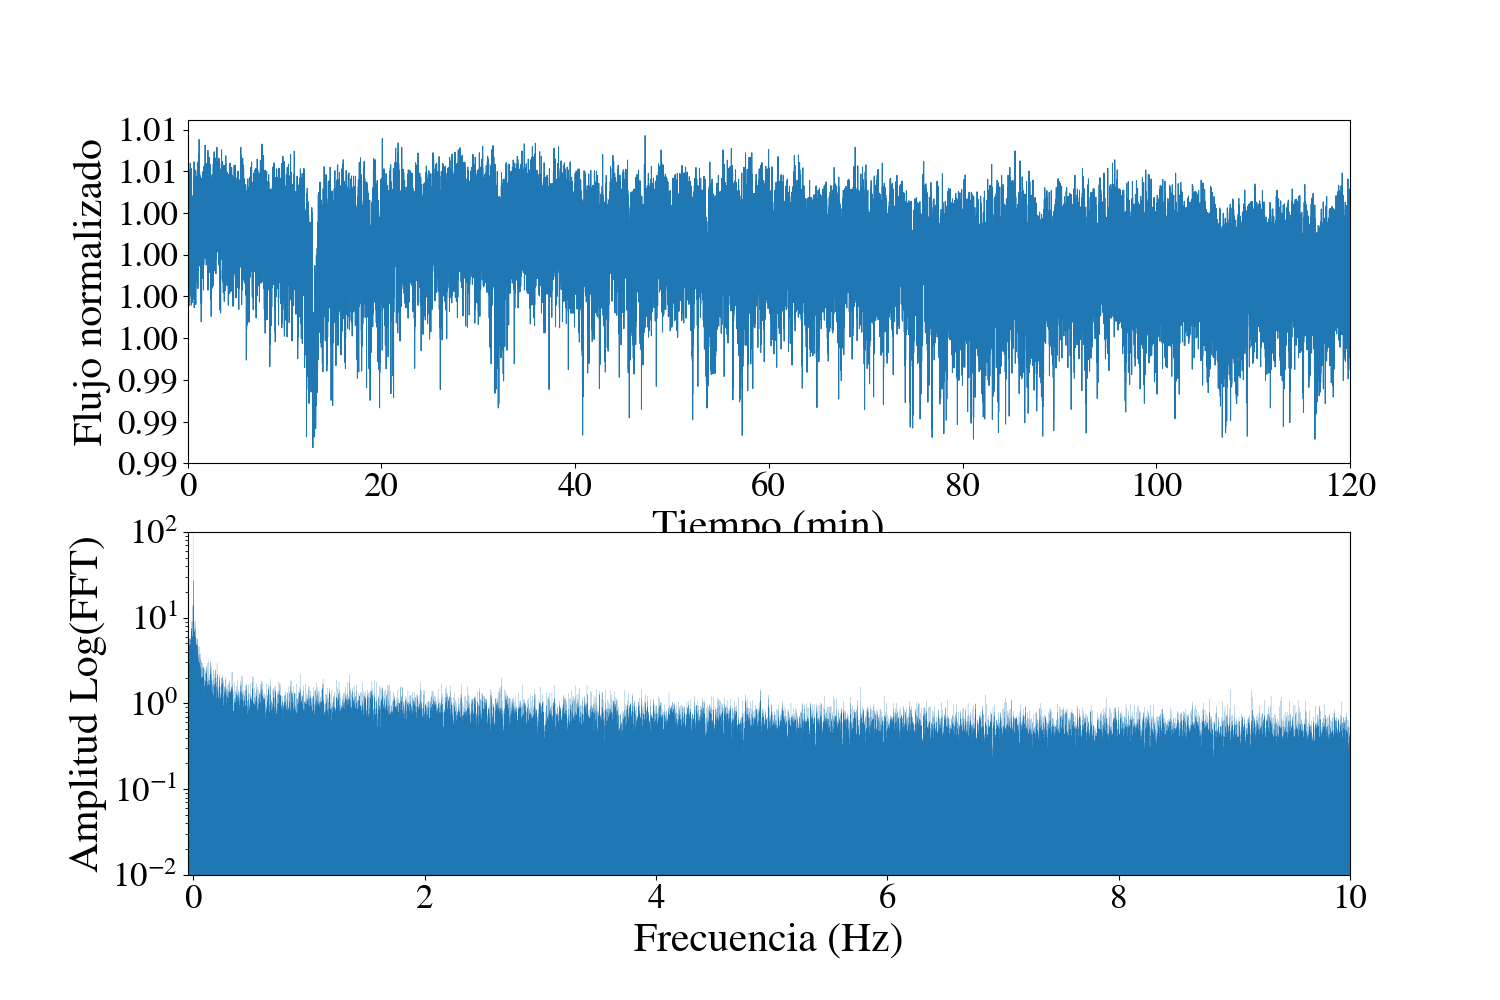
\includegraphics[max size={\textwidth}{0.6\textheight}]{./figures/transformada_fourier.png}
   \caption{Arriba: Curva de luz de alta cadencia de HAT-p-14b, tomada a 20Hz, con el telescopio de 84cm del OAN. Abajo: mostramos su espectro de frecuencias (FFT), con la amplitud en escala logarítmica para mejorar la visualización.}
    \label{fig_2_9_fourier}
\end{figure}

En la figura 2.6 podemos apreciar una curva de luz de alta cadencia y su respectivo espectro de frecuencias. Como podemos observar, se aprecia una importante componente de bajas frecuencias debido a las tendencias en la curva de luz, provocadas por variables atmosféricas. Es por eso que en este trabajo se modeló el ruido de una manera en la que el ruido simulado tenga componentes que observamos en curvas de luz reales (véase III.2.2), a diferencia de simplemente añadir un ruido con distribución gaussiana (ruido blanco) el cual tiene un espectro de frecuencias plano.

En este trabajo se utilizó el análisis de Fourier para encontrar las componentes del ruido y limpiar la curva de luz con una metodología ágil y rápida \cite{kosarev1983optimal}, \cite{brault1971analysis}. U

\section*{II.6 Análisis de componentes principales}
\addcontentsline{toc}{section}{II.4 Análisis de componentes principales}

\textcolor{red}{ESTA SECCION DEBERIA IR DENTRO DE LA METODOLOGIA, EN LA PARTE DE PCA, AQUÍ ESTÁ DEMASIADO AISLADA, A MENOS QUE SE INCLUYA AQUÍ TODO LO DE PROMEDIO MOVIL Y FILTRADO DE FOURIER}

Para toda matriz $A$ con dimensiones $m\times n$, su descomposición en valores singulares ó SVD (del inglés \textit{Singular Value Decomposition}) es:

\begin{equation}
  \displaystyle A=U\Sigma V^{T};
\end{equation}

\noindent donde:\\

\begin{itemize}
  \item $U$ es llamado \textit{vector singular} y es ortogonal $(UU^{T}=I)$,
  \item $\Sigma$ está compuesta por los valores singulares de $U$ y es diagonal no negativa,
  \item $V$ es también un \textit{vector singular} y es ortogonal $(VV^{T}=I)$.
\end{itemize}

Si multiplicamos la ecuación 2.14 por su transpuesta tenemos:

\begin{equation}
  \displaystyle AA^{T}=U\Sigma V^{T} V\Sigma U^{T} = U \Sigma^{2} U^{T};
\end{equation}

\noindent el resultado es el conocido teorema de diagonalización para matrices simétricas que dice: \textit{Sea S una matriz cuadrada de $M\times M$ con $M$ eigenvectores linealmente independientes, entonces existe una descomposición simétrica tal que:}

\begin{equation*}
  \displaystyle S=Q\Lambda Q^{T};
\end{equation*}


\noindent \textit{donde las columnas de $Q$ son los eigenvectores normalizados de $S$, y $\Lambda$ es la matriz diagonal con los eigenvalores de $S$.}

El significado matemático de la SVD, depende de la forma de $A$. Normalmente $A$ con dimensiones $m\times n$ está compuesta por los datos, donde $m$ es el número de muestras y $n$ el número de variables. Los \textit{vectores singulares} $U$, son también conocidos domo \textit{ejes principales} y la proyección de los datos $A$ sobre estos ejes principales son llamados \textit{componentes principales ($P_{comp}$)}, es decir $(P_{comp}=AU)$, de ahí el nombre de análisis de componentes principales ó PCA (del inglés \textit{Principal Component Analysis}).

Esta descomposición es utilizada para la extracción de características y disminuir la dimensionalidad de los datos que se estén analizando (\cite{mcgurk2010principal}; \cite{medeiros2018principal}). En este trabajo se utilizan las componentes principales para limpiar la curva de luz del ruido sistemático (\cite{shin1999iterative}; \cite{bailey2012principal}).